


\section{PDRベースの屋内位置推定\\ライブラリの検討}
本章では,屋内位置推定ライブラリの要求仕様の検討およびその実装について述べる。
節3.1では要求仕様について詳述する.
節3.2では,軌跡の画像と関数を用いて,どのような補正を行っているかを示す.



\subsection{要求仕様}                                      
PDRと他の情報を使ってライブラリを作成する上で,
どのような状況や環境が存在し補正に利用できるのかその具体的な例を考える必要がある.
例えば大学内や病院などのWi-FiのAPが多く設置されている場所では,
Wi-Fiの電波強度を利用した位置推定が有効である.
他の例として展示会場や大きなアトリウムなどの広い開放空間が考えられる.
このような場所ではWi-FiのAPの配置が難しく,
信号のカバレッジが不均一になりやすくWi-Fiを利用した位置推定は難しい.
このような場所の場合BLEビーコンを配置してその電波強度を利用した位置推定が有効である.
また2章で示したように\cite{pdr-wifi}\cite{pdr-ble}などのPDRと電波を利用した推定に関する研究は盛んに行われている.
このように電波を使った手法は多くの場所で有効であり,補正に利用可能な情報として重要度が高い.
そのため本ライブラリにおいても採用を行う.
他に補正に利用可能な情報としてフロアマップ情報がある.
フロアマップ情報は多くの場所で比較的入手が容易だと思われる.
そのため本ライブラリにおいても採用を行う.
磁気やカメラなどの情報は,磁気データはデータが繊細であり電波と比べると補正に利用する難易度が高い,
カメラはプライバシーの問題などの問題があり本ライブラリの基礎段階において採用しない.
また気圧センサは基礎段階として3次元空間を推定対象としないため採用しない.

本ライブラリの補正アルゴリズム実装の検討および,その有効性の検証においてxDR Challenge 2023\cite{xdr}の環境を用いる.
xDR Challenge 2023 はPDRベンチマーク委員会が主催する屋内位置推定の精度を競うコンテストである.
このコンテストでは主催者が参加者に対して複数の訓練データを提供する.
被験者は腰にスマートフォンをつけた状態で,LiDARと呼ばれる距離測定技術を搭載したハンドヘルドLiDARを持ちBLEビーコンが配置された高速道路のサービスエリア内を歩く.
この過程で取得されたデータが訓練データとして提供される.
LiDARからは歩行者のフロアマップにおける歩行者の初期位置,終了位置,移動経路のデータが提供される.
LiDARは光を使って物体や壁までの距離を精密に測定できる技術であり,
このコンテストではLiDARから得られる提供データを正解軌跡として扱っている.
スマートフォンからは加速度,角速度,地磁気,各BLEビーコンのAP情報と受信電波強度が提供される.
フロアマップ情報,各ビーコンのフロアマップにおける基地局の位置情報は事前にコンテスト主催者側によって提供される.
そしてこの提供されたデータを基にコンテスト参加者は独自の推定アルゴリズムの開発を行い位置推定を行う.
本番で与えられるデータは訓練データと同様のフロアマップのデータが提供されるが,
LiDARからのデータは初期位置と終了位置しか提供されず,それ以外の情報を使って歩行者の移動軌跡を推定する.
xDR Challenge 2023の環境は,フロアマップ情報,各ビーコンの情報,スマートフォンからのセンサデータが提供されており
PDRと他の情報を使用したPDRの補正が可能であり,本ライブラリの要求仕様に適合している.
またライブラリを用いた処理の結果どのような補正の効果が得られるのかを検証する必要がある.
XDR Challenge 2023の環境は後述する評価システムが確立されており,本ライブラリの有効性を検証する環境が整備されている.
よってこの環境を基に補正アルゴリズム実装の検討および有効性の検証を行う.



\subsection{ライブラリの実装}

\begin{table*}[ht]
	\caption{関数に必要な情報とその対応表} \label{}
	\textit{注: $\circ$は必須引数,$\triangle$はオプショナル引数を示す} \label{tab:my_label}
	\centering
	\scalebox{0.59}{
		\begin{tabular}{|c|c|c|c|c|c|c|c|c|c|c|c|c|c|} 
			\hline
			                   & 関数名                                                                 & \multicolumn{4}{c|}{センサ情報}   & \multicolumn{4}{c|}{環境情報}    & \multicolumn{4}{c|}{その他}                                                                                                                                                                                                                                                                                                                                 \\ \hline
			                   &                                                                     &                              &                              &                              & \multicolumn{1}{c|}{BLEビーコン} &                              & \makecell{磁気                                                                                                } & \multicolumn{2}{c|}{BLEビーコン} & \multicolumn{2}{c|}{正解初期}        & \multicolumn{2}{c|}{正解補正}                                                 \\ \cline{6-6} \cline{8-8} \cline{9-9} \cline{10-10}\cline{11-12}\cline{13-14}
			                   &                                                                     & 加速度                          & 角速度                          & 角度                           & 電波強度・AP情報                    & フロアマップ                       & FP                                                                                                            & 基地局位置                        & FP                               & 座標                               & 方向 & 座標                           & 方向 \\ \hline
			基本PDR              & estimate\_trajectory                                                & \multicolumn{1}{c|}{$\circ$} & \multicolumn{1}{c|}{$\circ$} &                              &                              &                              &                                                                                                               &                              &                                  & \multicolumn{1}{c|}{$\triangle$} &    &                              &    \\ \hline
			角速度から角度推定          & convert\_to\_angle\_from\_gyro                                      &                              & \multicolumn{1}{c|}{$\circ$} &                              &                              &                              &                                                                                                               &                              &                                  &                                  &    &                              &    \\ \hline
			ドリフト補正             & remove\_drift\_in\_angle                                            & \multicolumn{1}{c|}{$\circ$} &                              & \multicolumn{1}{c|}{$\circ$} &                              &                              &                                                                                                               &                              &                                  & \multicolumn{1}{c|}{$\circ$}     &    & \multicolumn{1}{c|}{$\circ$} &    \\ \hline
			初期進行方向補正 歩行可能領域マップ & rotate\_trajectory\_to\_optimal\_alignment\_using\_map              & \multicolumn{1}{c|}{$\circ$} &                              & \multicolumn{1}{c|}{$\circ$} &                              & \multicolumn{1}{c|}{$\circ$} &                                                                                                               &                              &                                  & \multicolumn{1}{c|}{$\triangle$} &    &                              &    \\ \hline
			初期進行方向補正 BLE       & rotate\_trajectory\_to\_optimal\_alignment\_using\_ble              & \multicolumn{1}{c|}{$\circ$} &                              & \multicolumn{1}{c|}{$\circ$} & \multicolumn{1}{c|}{$\circ$} &                              &                                                                                                               & \multicolumn{1}{c|}{$\circ$} &                                  & \multicolumn{1}{c|}{$\triangle$} &    &                              &    \\ \hline
			マップマッチング補正         & move\_unwalkable\_points\_to\_walkable                              & \multicolumn{1}{c|}{$\circ$} &                              & \multicolumn{1}{c|}{$\circ$} &                              & \multicolumn{1}{c|}{$\circ$} &                                                                                                               &                              &                                  & \multicolumn{1}{c|}{$\triangle$} &    &                              &    \\ \hline
			初期進行方向補正 BLE FP    & rotate\_trajectory\_to\_optimal\_alignment\_using\_ble\_fingerprint
			                   & \multicolumn{1}{c|}{$\circ$}                                        &                              & \multicolumn{1}{c|}{$\circ$} &                              &                              &                              &                                                                                                               & \multicolumn{1}{c|}{$\circ$} & \multicolumn{1}{c|}{$\triangle$} &                                  &    &                                   \\ \hline
		\end{tabular}
	}
\end{table*}


関数に必要な引数の情報をいくつかの種類に分類し,それを各関数に対応づけたものを表1に示す.
詳しい関数の説明や内部実装については後述する.
引数の情報は大きく分けてセンサ情報,環境情報,その他の3つに分類される.
センサ情報はスマートフォンから得られる加速度,角速度,BLEビーコンの電波情報などが含まれる.
環境情報はフロアマップ,フロアマップにおける各BLEビーコンの配置情報などが含まれる.
これらの環境情報は全てセンサデータが与えられる前に得られる情報である.
その他はセンシング中,またはセンシング前に得られる情報であり,初期位置,終了位置などの情報が該当する.

本ライブラリの実装にはプログラミング言語PythonとそのライブラリであるPandasを主に使用した.
Pythonには科学技術関連ライブラリが豊富に存在し,Numpy,Pandas,Scikit-learn,Matplotlibなどデータ分析や機械学習を支援する強力なライブラリがある.
特にPandasライブラリはデータ解析を容易にする多くの機能を提供している.
Pandasはデータフレーム(以下,DF)と呼ばれるデータ構造を提供し,
DFは表形式のデータを扱うための強力なツールであり,
行と列から構成される2次元のデータ構造である.
PandasはDFの操作を容易にする機能を提供し,
これにより大量のセンサデータを効率的に操作・分析できる.
これは本ライブラリ内部処理において必要なデータの読み込み,集約,フィルタリングといった操作に適している.
そのため本ライブラリの引数や内部処理のデータ構造にもPandasのDFが使用されている.

まず基本的なPDRの処理を行う関数をListing\ref{lst:pdr-trajectory}に示す.
この関数では加速度DF,角速度DFを使用して位置推定を行う.
加速度DF,角速度DFのデータフレームのカラム名とデータ型を表2,表3に示す.
オプショナル引数として正解初期座標(ground\_truth\_first\_point)を与えられる.
正解初期座標は辞書型で表4に示す.
戻り値は時間経過に伴う2次元座標のDF(以下,座標DF)と角度DFであり,それぞれのカラム名とデータ型を表5,表6に示す.
戻り値として角度DFを返しているのは各補正関数が角度DFを引数として受け取る設計なためである.
各補正関数は内部で角度DFを使用し処理を行っており,角速度DFを引数として受け取る場合に比べ,積分処理を省略できる利点がある.

\begin{table}[ht]
	\caption{加速度 DF}
	\centering
	\begin{tabular}{lll}
		\toprule
		カラム名 & 単位        & データ型  \\
		\midrule
		ts   & s (秒)     & float \\
		x    & m/s\(^2\) & float \\
		y    & m/s\(^2\) & float \\
		z    & m/s\(^2\) & float \\
		\bottomrule
	\end{tabular}
\end{table}

\begin{table}[ht]
	\caption{角速度 DF}
	\centering
	\begin{tabular}{lll}
		\toprule
		カラム名 & 単位             & データ型  \\
		\midrule
		ts   & s (秒)          & float \\
		x    & rad/s (ラジアン/秒) & float \\
		y    & rad/s (ラジアン/秒) & float \\
		z    & rad/s (ラジアン/秒) & float \\
		\bottomrule
	\end{tabular}
\end{table}


\begin{table}[ht]
	\caption{正解初期座標 DICT}
	\centering
	\label{tab:first-coord-dict}
	\begin{tabular}{lll}
		\hline
		      & {データ型}         & {説明}          \\ \hline
		key   & \texttt{str}   & xまたはy         \\ \hline
		value & \texttt{float} & \makecell{座標} \\ \hline
	\end{tabular}
\end{table}


\begin{table}[ht]
  \caption{時間経過に伴う2次元座標DF(座標DF)}
	\centering
	\begin{tabular}{lll}
		\toprule
		カラム名 & 単位      & データ型  \\
		\midrule
		ts   & s (秒)   & float \\
		x    & m(メートル) & float \\
		y    & m(メートル) & float \\
		\bottomrule
	\end{tabular}
\end{table}


\begin{table}[ht]
  \caption{角度 DF}
	\centering
	\begin{tabular}{lll}
		\toprule
		カラム名 & 単位         & データ型  \\
		\midrule
		ts   & s (秒)      & float \\
		x    & rad (ラジアン) & float \\
		y    & rad (ラジアン) & float \\
		z    & rad (ラジアン) & float \\
		\bottomrule
	\end{tabular}
\end{table}


本ライブラリの実装では歩幅や歩行タイミングの正確な推定を行わない.
歩幅の推定を行っている研究は多くある.
機会学習を用いた研究\cite{stride-length-auto-learning},
多変量解析を用いた研究\cite{stride-length-multi},
超音波センサーガジェットを用いた研究\cite{stride-length-ultrasonic}などがある.
本関数の内部処理では歩幅の値は固定値として扱っている.
本来であれば歩幅は身長,性別,年齢などの複数の要素によって動的に変化するため
固定値なのはありえず,先ほど挙げた研究のように歩幅を推定する必要がある.
しかし本ライブラリの目的は正確な歩幅を用いたPDRによる位置推定ではない.
そのため歩幅の推定は行わず固定値として扱う.
また同様の理由で歩行タイミングの検出も正確には行わず,加速度の値が特定の閾値を超えた時を
歩行タイミングとして扱っている.

xDR Challenge 2023で与えられたトレーニングデータの
一部に対してライブラリを用いて位置推定を行いそれが
どのように変更されるのか図を用いて示していく.
図\ref{fig:pdr}にListing\ref{lst:pdr-trajectory}を用いてPDRによる位置推定を行った結果を示す.
この図は2次元座標上に推定軌跡を表し,カラーバーが経過時間を表している.
LiDARで取得した座標を基に出力された軌跡を図\ref{fig:gt-trajectory}に示す.
これを本論では正解軌跡とする.
図\ref{fig:pdr}と図\ref*{fig:gt-trajectory}を比較するとPDRによる軌跡は正解軌跡と比べて大きくずれているのがわかる.
PDR特有の解決すべきものとして
軌跡そのものの形状を正解奇跡に近づける問題と絶対位置との関連付けの問題がある.
本ライブラリを用いてこれらの問題を解消し正解軌跡に近づけていく.
Listing\ref{lst:pdr-trajectory}に示される関数に正解初期座標を
を与えたのが図\ref{fig:pdr-move}である.
予め正解座標が判明している場合はPDRによる軌跡の初期位置を補正できる.



% 文書内
\begin{lstlisting}[caption={基本PDR}, label=lst:pdr-trajectory]
Axis2D = Literal["x", "y"]
def estimate_trajectory(
    acc_df: pd.DataFrame,
    gyro_df: pd.DataFrame,
    *,
    ground_truth_first_point: dict[Axis2D, float] | None = None,
) -> tuple[pd.DataFrame, pd.DataFrame]:
\end{lstlisting}

\begin{figure}[ht]
	\centering
	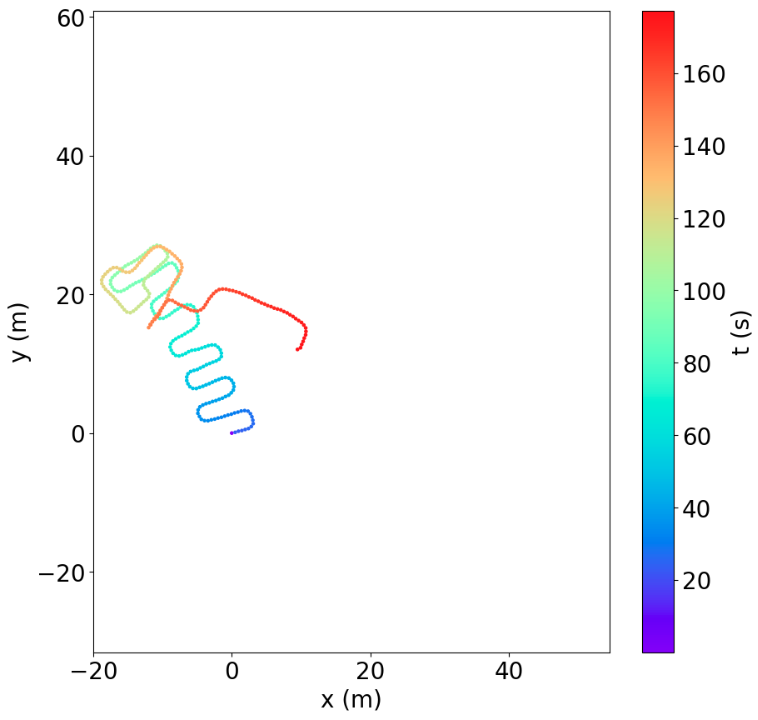
\includegraphics[width=80mm]{image/pdr.jpg}
	\caption{基本PDRの軌跡}    \label{fig:pdr}
\end{figure}

\begin{figure}[ht]
	\centering
	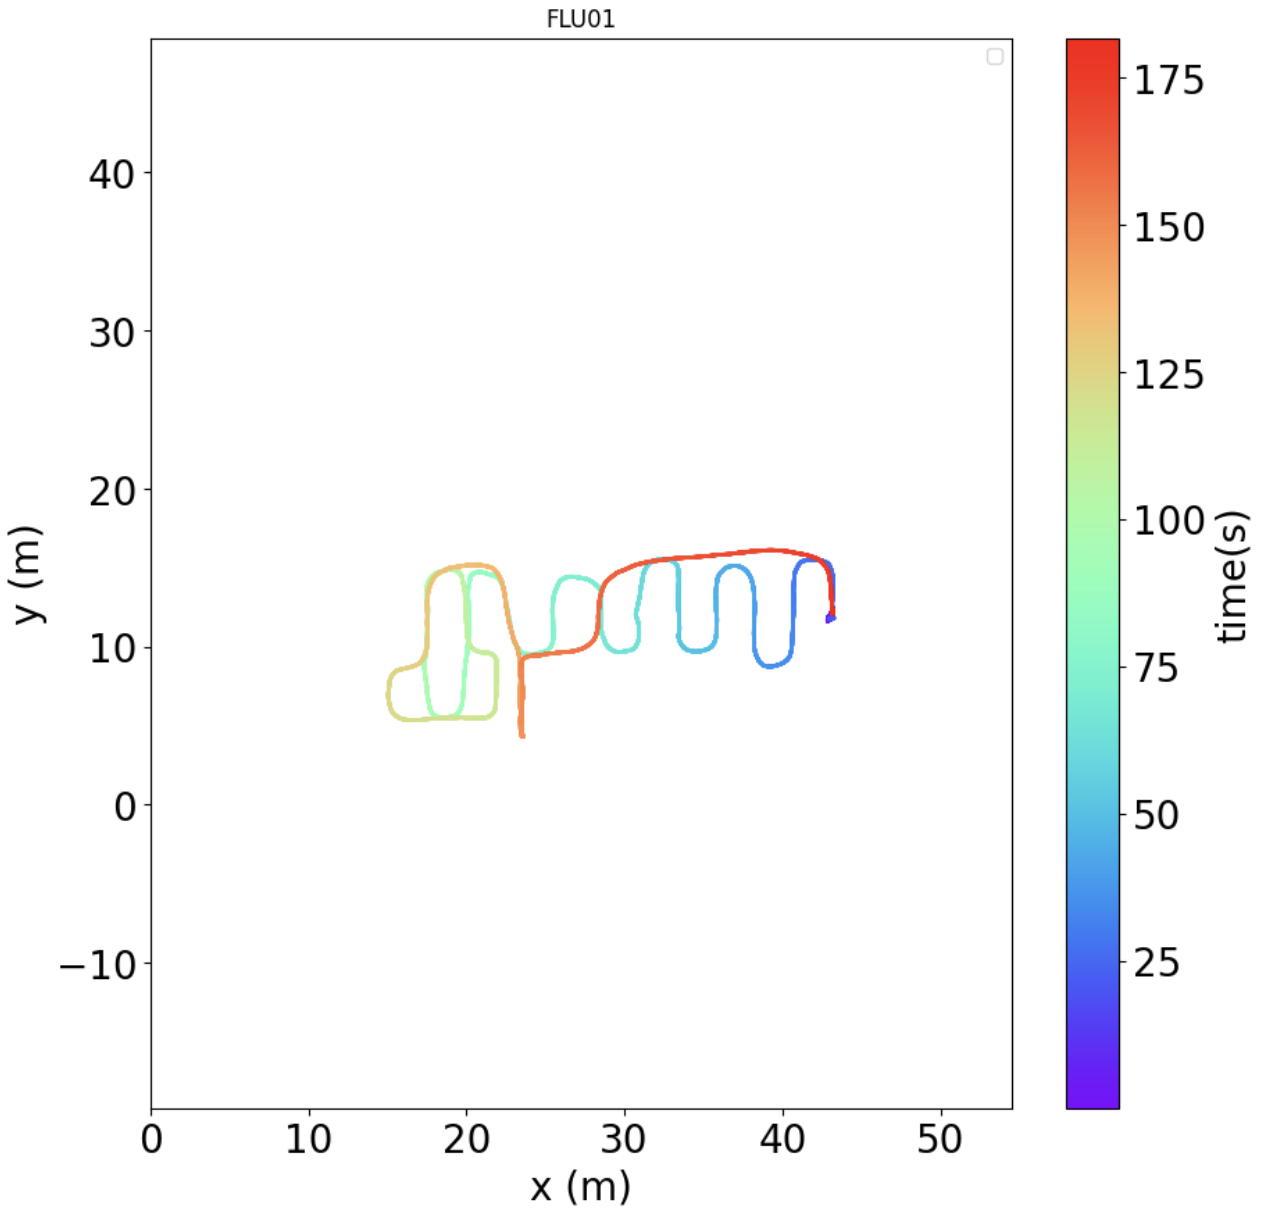
\includegraphics[width=80mm]{image/gt2.jpg}
	\caption{正解軌跡}    \label{fig:gt-trajectory}
\end{figure}

\begin{figure}[ht]
	\centering
	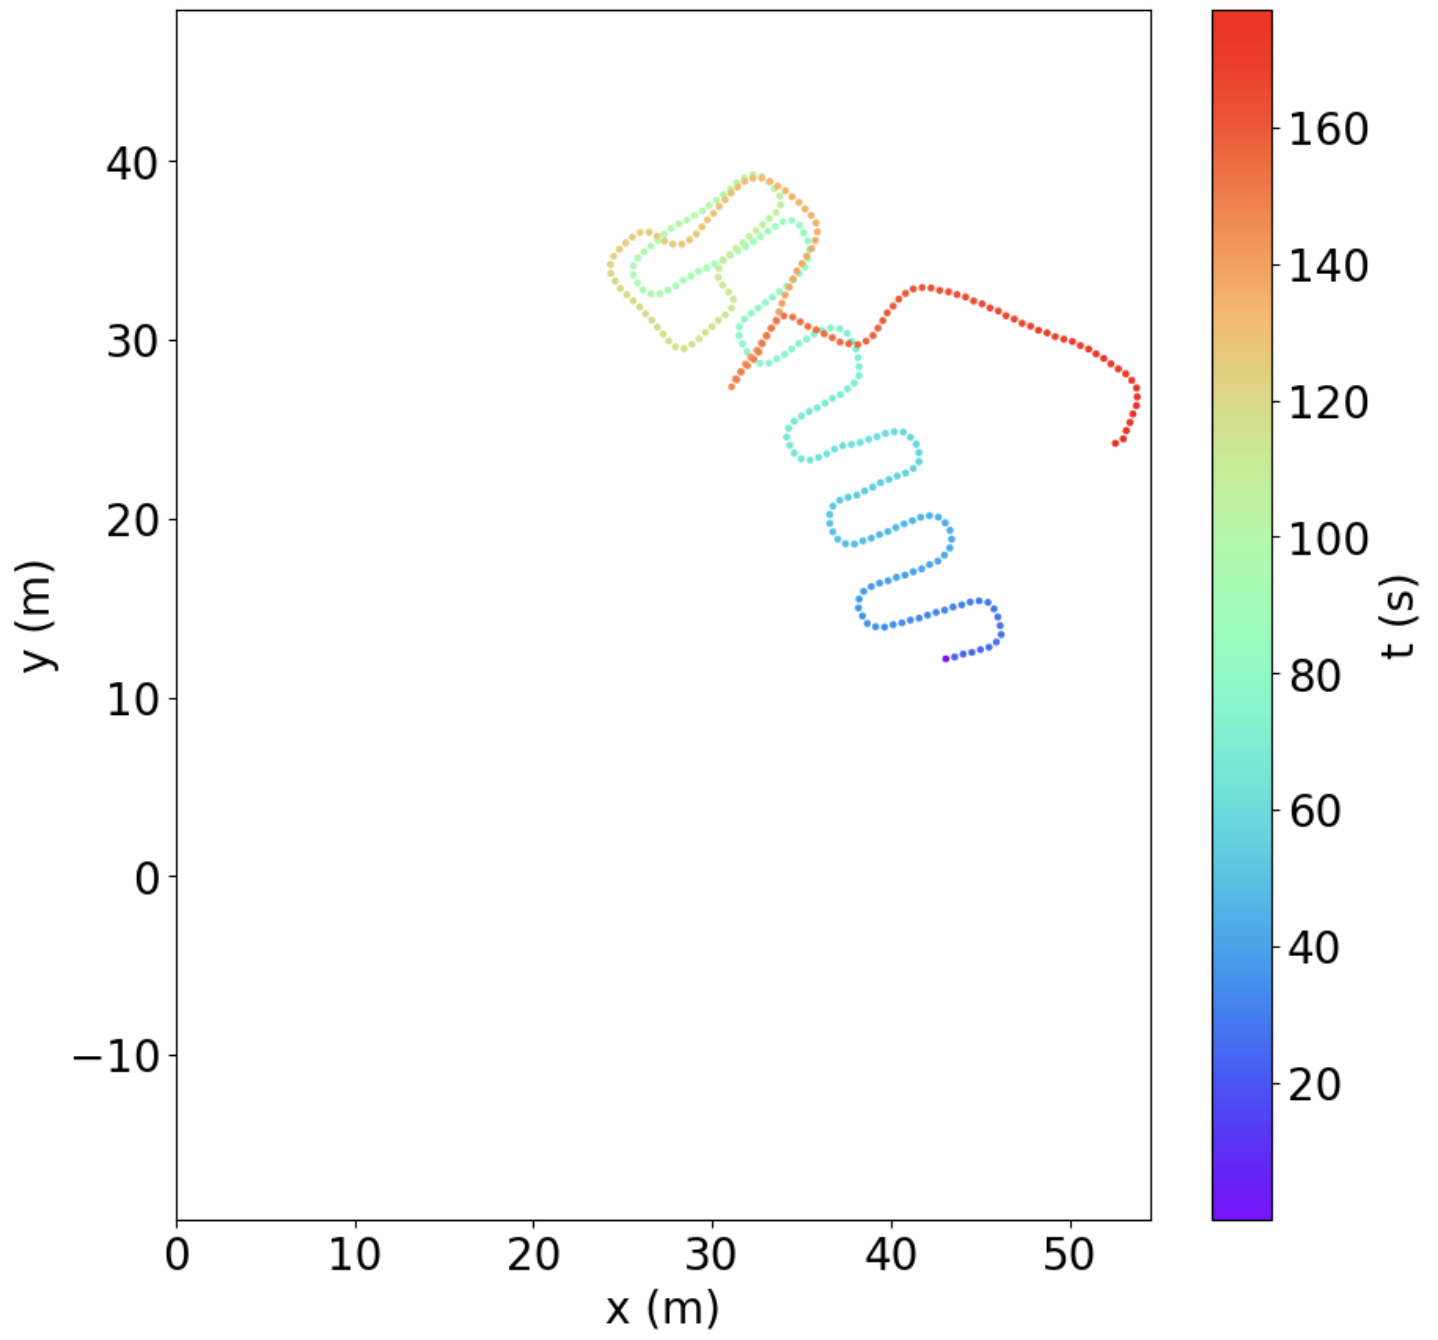
\includegraphics[width=80mm]{image/pdr-move.jpg}
	\caption{正解初期座標が存在}    \label{fig:pdr-move}
\end{figure}







図\ref{fig:pdr-move}の軌跡にはPDR特有のドリフト現象が見られる.
PDRでは角速度から進行方向を求めてその方向を元に歩行軌跡を描く.
そのため角速度センサーにわずかなでも誤差が含まれると時間経過とともにその誤差が大きくなり軌跡の形状が本来の軌跡から外れる.
この問題を解決するには角速度データに含まれる累積誤差を取り除く必要がある.


\begin{lstlisting}[caption={ドリフト除去}, label=lst:remove-drift]
def remove_drift_in_angle_df(
    acc_df: pd.DataFrame,
    angle_df: pd.DataFrame,
    ground_truth_point_df: pd.DataFrame,
) -> tuple[pd.DataFrame, pd.DataFrame]:
\end{lstlisting}

ドリフトを取り除く関数をListing\ref{lst:remove-drift}に示す.
引数として加速度DF,角速度DF,正解座標DFを受け取る.
戻り値は角度DFと座標DFを返す.
ドリフト補正のプロセスは,ドリフトの値を動的に計算し,それを各時刻の角度データから差し引く.
このドリフト補正プロセスは,式(1)で表される.
$\theta'(t)$は時間$t$における補正後の角度,$\theta(t)$は補正前の角度,
$\mathrm{d}$はドリフトの大きさを意味する.
この式は時間経過に伴うドリフトの累積効果を補正するために使用される.


\vspace{5mm} % 5mmの空白を追加。必要に応じて値を調整してください。
\begin{equation}
	\theta'(t) = \theta(t) - (\mathrm{d} \times (t))
\end{equation}

\vspace{5mm} % 5mmの空白を追加。必要に応じて値を調整してください。

補正の効果を評価し適切なドリフトを見つけるために,ユークリッド距離を用いて,2つの正解座標の差異を計算する.
式(2)は,正解座標$(x_{\mathrm{n}}, y_{\mathrm{n}})$と正解座標$(x_{\mathrm{n+1}}
	y_{\mathrm{n+1}})$との間のユークリッド距離$\mathrm{E}$を示している.
この式に基づきドリフト値に対してグリッドサーチを行い距離が最小になるドリフト値を探す.
最小のドリフト値を角度DFから引きそれに基づいた座標DFと角度DFを返す.
図\ref{fig:pdr-remove-drift}に示すように,ドリフト補正後の軌跡は,元の軌跡と比較して正解軌跡の形状に近づいている.
このアルゴリズムでは正解座標$(x_{\mathrm{n}}, y_{\mathrm{n}})$と
正解座標$(x_{\mathrm{n+1}}, y_{\mathrm{n+1}})$の距離が近い時に特に有効である.
この処理は$(x_{\mathrm{n+2}}, y_{\mathrm{n+2}})$など2つ以上の座標が存在する場合も同様に適用できる.

\vspace{5mm} % 5mmの空白を追加。必要に応じて値を調整してください。
\begin{equation}
	\mathrm{E} = \sqrt{(x_{\mathrm{n+1}} - x_{\mathrm{n}})^2 + (y_{\mathrm{n+1}} - y_{\mathrm{n}})^2}
\end{equation}
\vspace{5mm} % 5mmの空白を追加。必要に応じて値を調整してください。

\begin{figure}[h]
	\centering
	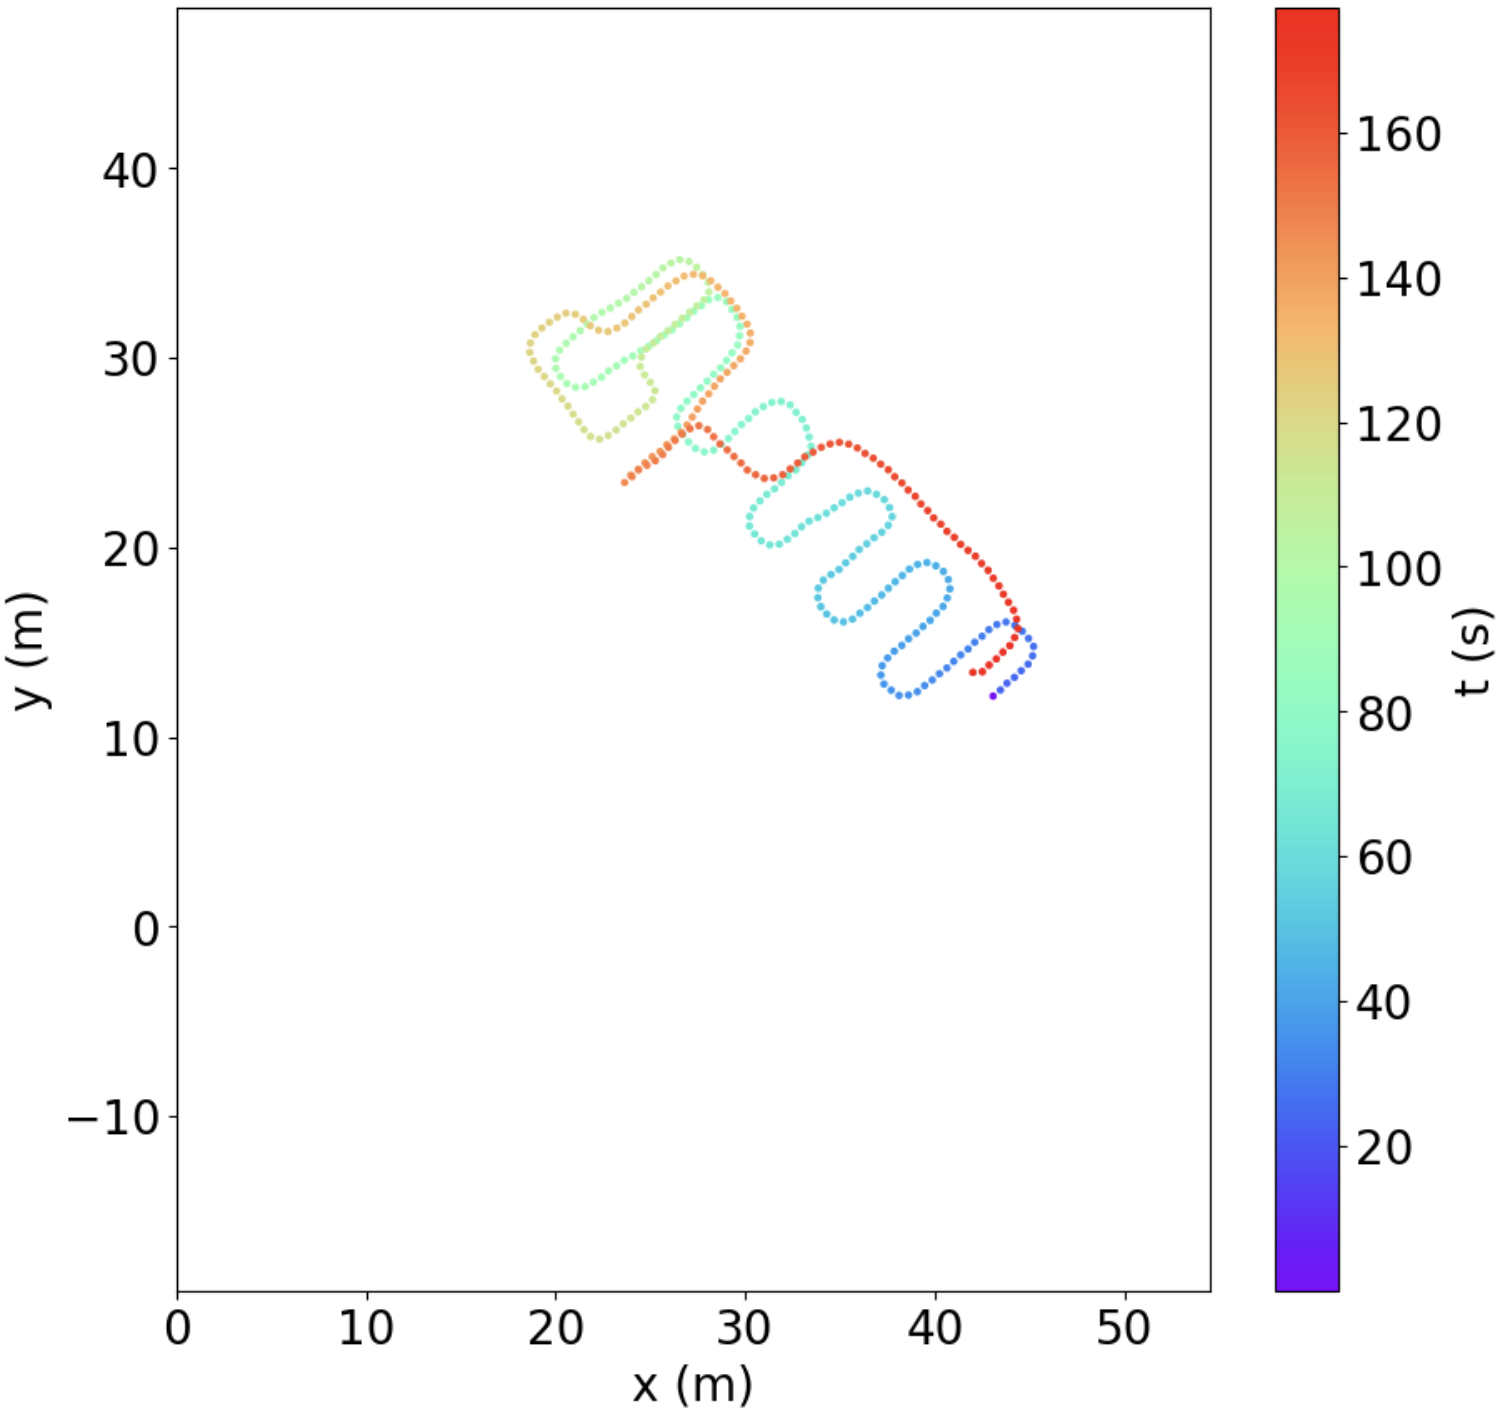
\includegraphics[width=80mm]{image/pdr-remove-drift-two.jpg}
	\caption{ドリフト補正後の軌跡}    \label{fig:pdr-remove-drift}
\end{figure}


図\ref{fig:pdr-remove-drift}の軌跡の問題点として初期進行方向の誤差がある.
初期進行方向が誤っていると,歩行者の実際の移動経路と大きく異なる軌跡になる.
この問題を解決するためには,適切な初期進行方向を見つけて軌跡全体を回転させる必要がある.
フロアマップ情報を元に軌跡を回転させる関数をListing\ref{lst:pdr-rotate}に示す.
引数として加速度DF,角度DF,表\ref{tab:map-dict}に示すフロアマップ情報DICT,フロア名,マップの1pxあたりの距離を受け取る.
実際に関数に与えられるサンプルデータのフロアマップを図\ref{fig:floor-map}に示す.
内部の処理としては軌跡を回転させx軸,y軸に平行な成分の割合を計算する.
それを可視化したものが図\ref{fig:color}である.
この割合が最も大きい回転角度をグリッドサーチを用いて探し最適な角度を見つける.
しかしこの処理だけでは適切な初期進行方向は絞り込めない.
割合が大きいものがあっても90度回転させるごとに水平垂直方向の割合が同一になるため,
4つの角度から適切な初期進行方向を見つける必要がある.
この絞り込みの処理としてマップ上の通行可能,不可能な座標の情報を利用する.
各回転角度での軌跡座標がマップ上で通行可能なポイントの数を計算し最も多いポイントを持つ回転角度を選択する.
この処理を適用した結果が図\ref{fig:pdr-rotate}である.
補正前と比べて軌跡の初期進行方向が正解軌跡に近づいている.

\begin{figure}[ht]
  \caption{関数に与えられるフロアマップ情報} \label{fig:floor-map}
	\centering
	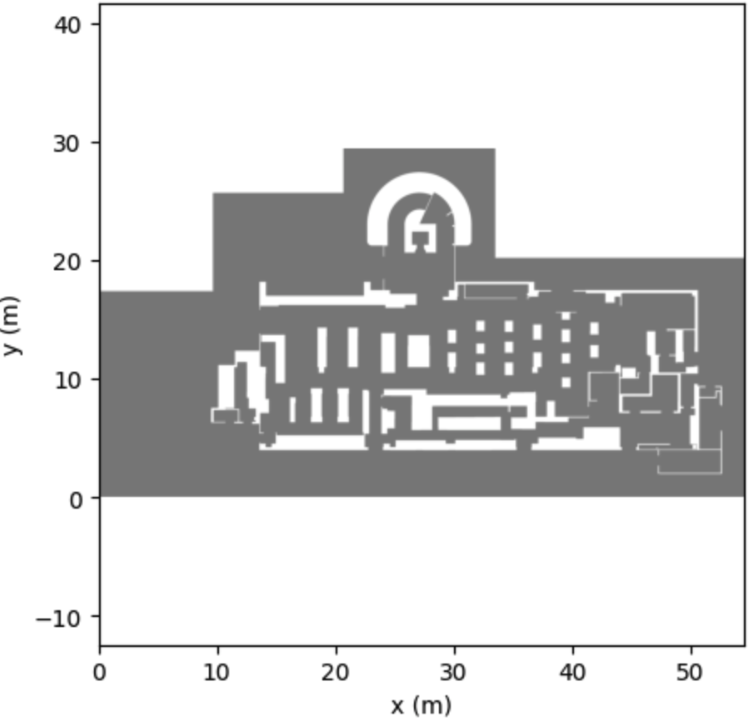
\includegraphics[width=80mm]{image/floor-map.jpg}
\end{figure}


\begin{lstlisting}[caption={初期進行方向補正}, label=lst:pdr-rotate,float =h]
def rotate_trajectory_to
		_optimal_alignment_using_map(
    acc_df: pd.DataFrame,
    angle_df: pd.DataFrame,
    map_dict: dict[str, np.ndarray],
    floor_name: str,
    dx: float,
    dy: float,
    *,
    ground_truth_first_point: dict[Axis2D, float] | None = None,
) -> tuple[pd.DataFrame, pd.DataFrame]:
\end{lstlisting}

\begin{table}[ht]
	\centering
	\begin{tabular}{lll}
		\hline
		      & \textbf{データ型}       & \textbf{説明}             \\ \hline
		key   & \texttt{str}        & floorの名前                \\ \hline
		value & \texttt{np.ndarray} & \makecell{フロアマップの画像データ. \\各フロアのブール値の\\NumPy配列} \\ \hline
	\end{tabular}
	\caption{フロマップ DICT}
	\label{tab:map-dict}
\end{table}

\begin{figure}[ht]
	\centering
	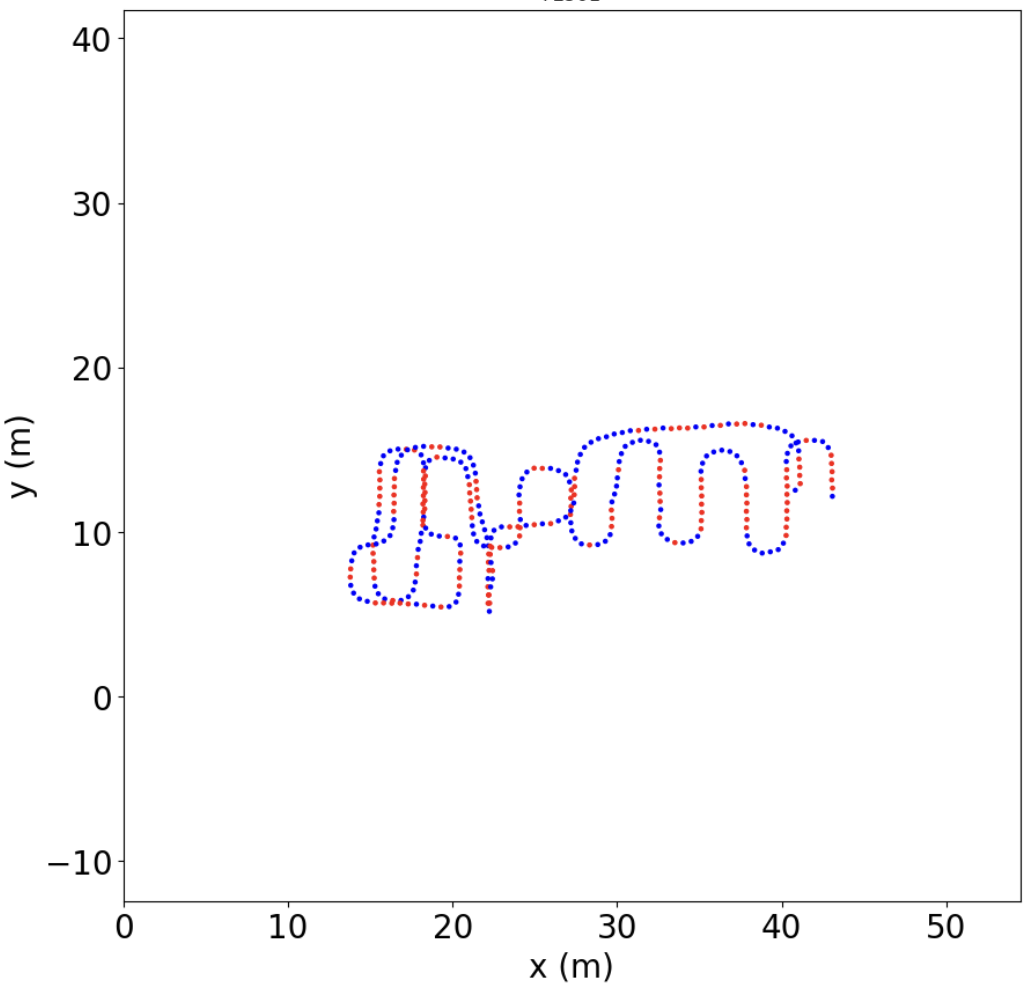
\includegraphics[width=80mm]{image/rb.jpg}
	\caption{垂直成分と水平成分の可視化}    \label{fig:color}
\end{figure}

\begin{figure}[ht]
	\centering
	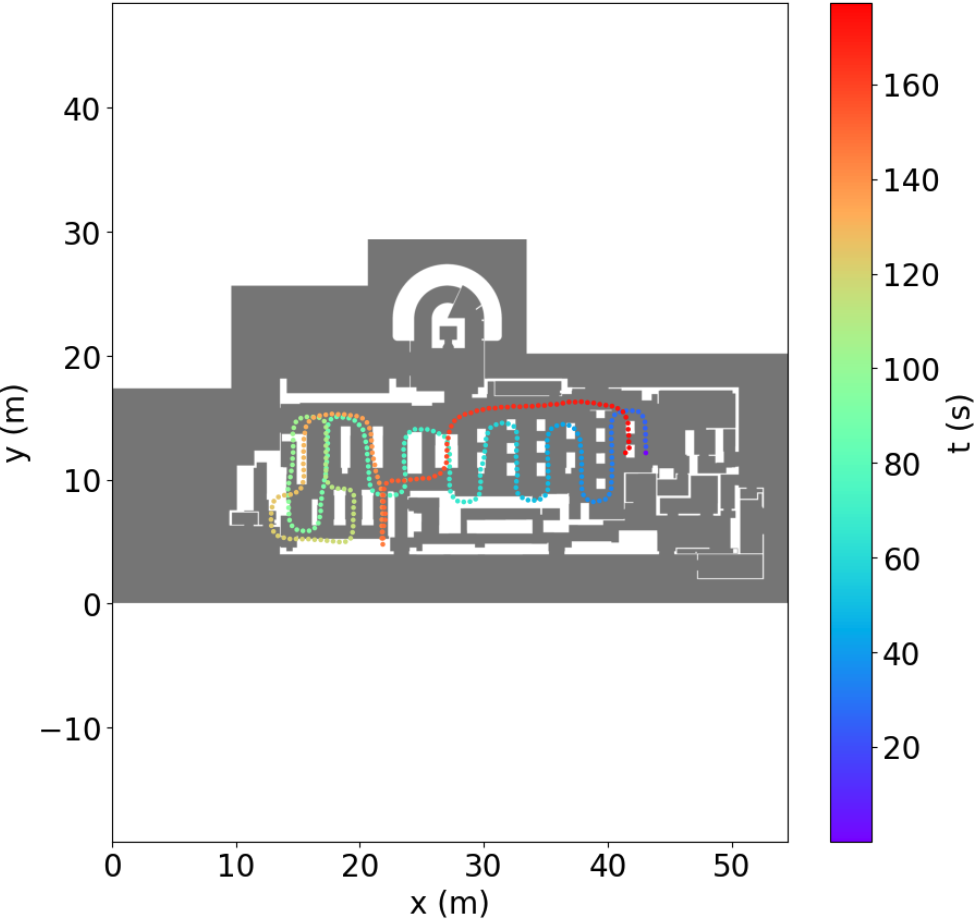
\includegraphics[width=80mm]{image/pdr-rotate.jpg}
	\caption{初期進行方向の補正後の軌跡}    \label{fig:pdr-rotate}
\end{figure}



フロアマップ情報を用いた初期進行方向補正ではマップの
存在可能な点の分布によっては正しく機能しない場合があり,
別の方法としてBLEビーコンの基地局の位置情報を用いた
初期進行方向補正を行う関数を提供する.関数をListing\ref{lst:rotate-trajectory-using-ble}に示す.
この関数では加速度DF,角度DF,BLEビーコンの受信電波DF, BLEビーコンの基地局DFを受け取る.
BLEビーコンの受信電波DFとBLEビーコンの基地局DFのカラム名とデータ型を表6,表7に示す.
戻り値は角度DFと座標DFを返す.
フロアマップ上に存在するBLEビーコン全ての基地局
一定の強いRSSIの電波を受信した際の時間情報を元に時間的に近い推定軌跡の座標を取得する.
図\ref{fig:ble-merge}に示した図は時間的に近い推定軌跡の座標を時間経過に応じた色で表しており
青色の座標が配置されたBLEビーコンの座標を表している.
推定した軌跡の受信したBLEビーコンの基地局の座標との距離を計算する.
この総和が最小となるような回転角度をグリッドサーチで探し最適な角度に補正を行う.
BLEビーコンの基地局の座標との距離を計算する.

\begin{lstlisting}[caption={BLEビーコンの基地局の位置情報を使用した初期進行方向補正}, label=lst:rotate-trajectory-using-ble]
def rotate_trajectory_to_optimal
		_alignment_using_ble(
    acc_df: pd.DataFrame,
    angle_df: pd.DataFrame,
    ble_scans_df: pd.DataFrame,
    ble_position_df: pd.DataFrame,
    *,
    ground_truth_first_point: dict[Axis2D, float] | None = None,
) -> tuple[pd.DataFrame, pd.DataFrame]:
\end{lstlisting}


\begin{figure}[ht]
	\centering
	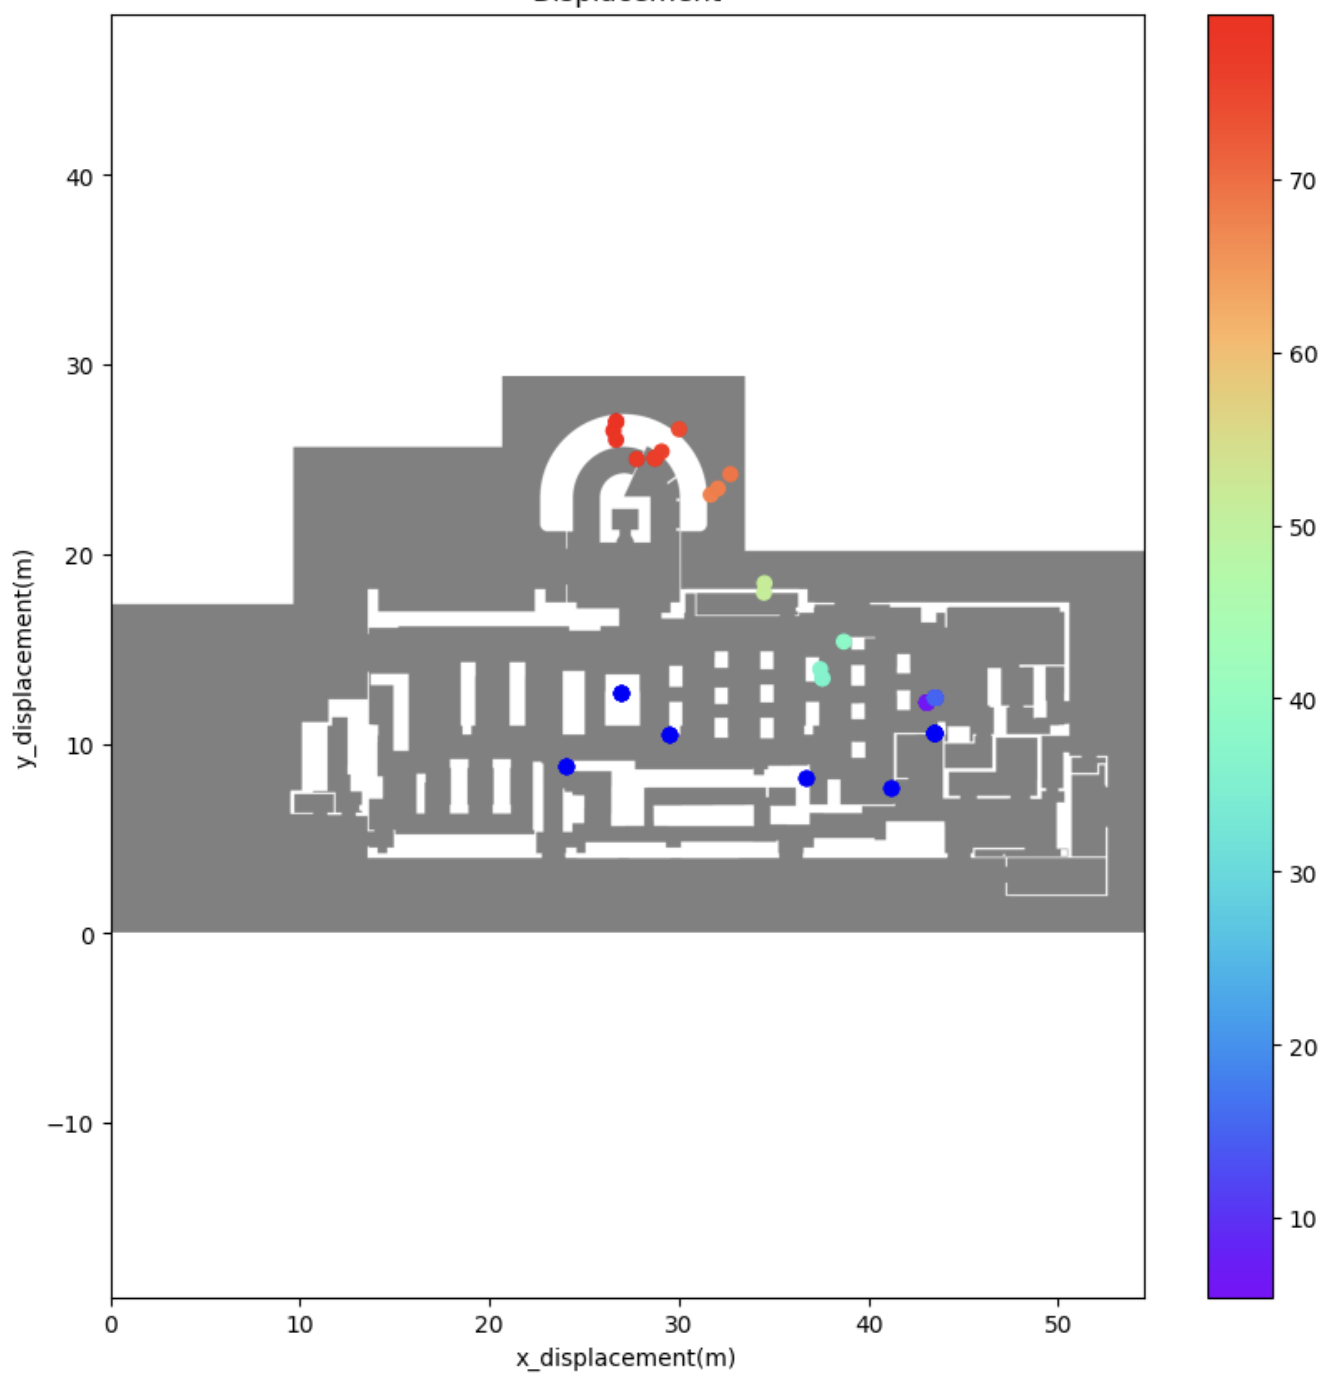
\includegraphics[width=80mm]{image/ble-merge.jpg}
	\caption{強いビーコン電波を受信した際の\\時間的に近い軌跡の座標}    \label{fig:ble-merge}
\end{figure}

\begin{table}[ht]
	\centering
	\begin{tabular}{lll}
		\toprule
		カラム名      & 単位    & データ型  \\
		\midrule
		ts        & s (秒) & float \\
		bdaddress & なし    & str   \\
		rssi      & dBm   & int   \\
		\bottomrule
	\end{tabular}
	\caption{BLEビーコン受信電波 DF}
\end{table}

\begin{table}[ht]
	\centering
	\begin{tabular}{lll}
		\toprule
		カラム名        & 単位 & データ型  \\
		\midrule
		bdaddress   & なし & str   \\
		x           & m  & float \\
		y           & m  & float \\
		floor\_name & なし & str   \\
		\bottomrule
	\end{tabular}
	\caption{BLEビーコン基地局 DF}
\end{table}

BLEビーコンの基地局の位置情報を基に初期進行方向の補正を行ったが
常にそれが利用可能であるとは限らない.
電波を使った手法としてWi-Fiを使った手法もあるがこの場合も同様であり
基地局の位置情報の把握にはコストがかかる場合がある.
基地局の位置情報を用いない代替手法としてFPを用いた手法がある.
この手法は,事前に特定の場所で受信したBLEビーコンのIDと
電波強度のデータを蓄積しておく必要があり,そのデータを基に
受信したIDとRSSIの値から位置を推定する.
この手法を用いて初期進行方向を補正する関数を
Listing\ref{lst:rotate-trajectory-using-ble-fingerprint}に示す.
この関数は引数に加速度DF,角度データDF,BLEビーコンの受信電波DF,
BLEビーコンのFPDF,フロア名を受け取る.
戻り値は角度DFと座標DFを返す.
受信電波情報とFPを基に推定した座標を示したのが図\ref{fig:fingerprint-location}である.
図の青色の点が受信したBLEビーコンの基地局座標であり,
赤色の点がこの基地局から受信した電波とFPを基に位置を推定した座標である.
理解しやすいように図中では受信したIDが1つのみを表示しているが,
実際は複数の強い電波を受信した点が存在する.
また説明のために基地局情報を示しているが今回の使用ケースでは
この座標は判明していないのが前提である.
この関数の内部処理では上記で示した受信電波情報とFPを基に推定した座標と
推定軌跡の座標との距離の総和を用いて,
その和が最小となる角度を探す.
BLEビーコンの基地局情報を基に初期進行方向を回転させた際と,ほぼ同様の結果が得られた.


\begin{table}[ht]
	\centering
	\begin{tabular}{lll}
		\toprule
		カラム名        & 単位      & データ型  \\
		\midrule
		ts          & s (秒)   & float \\
		x           & m(メートル) & float \\
		y           & m(メートル) & float \\
		z           & m(メートル) & float \\
		bdaddress   & なし      & str   \\
		rssi        & dBm     & int   \\
		floor\_name & なし      & str   \\
		\bottomrule
	\end{tabular}
	\caption{BLEビーコンFPのDF}
	\label{table:ble-beacon-fingerprint-df}
\end{table}


\begin{figure}[ht]
	\centering
	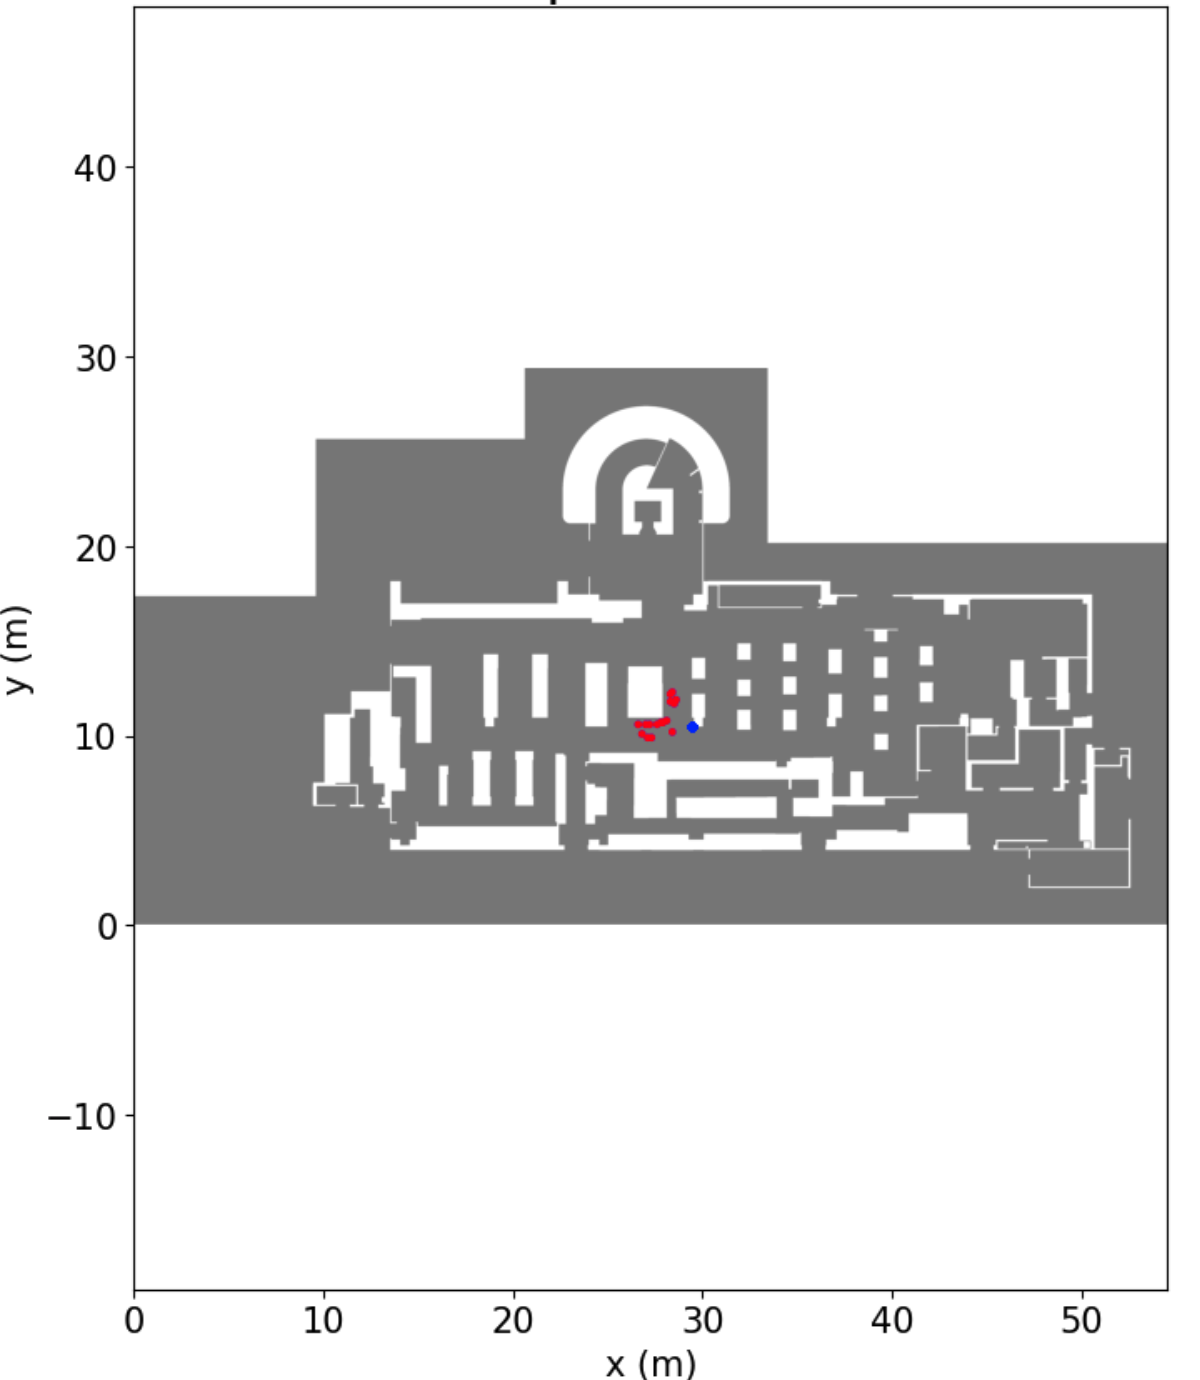
\includegraphics[width=80mm]{image/fingerprint-location.jpg}
	\caption{FPに基づく位置の推定}    \label{fig:fingerprint-location}
\end{figure}


\begin{figure}[ht]
	\centering
	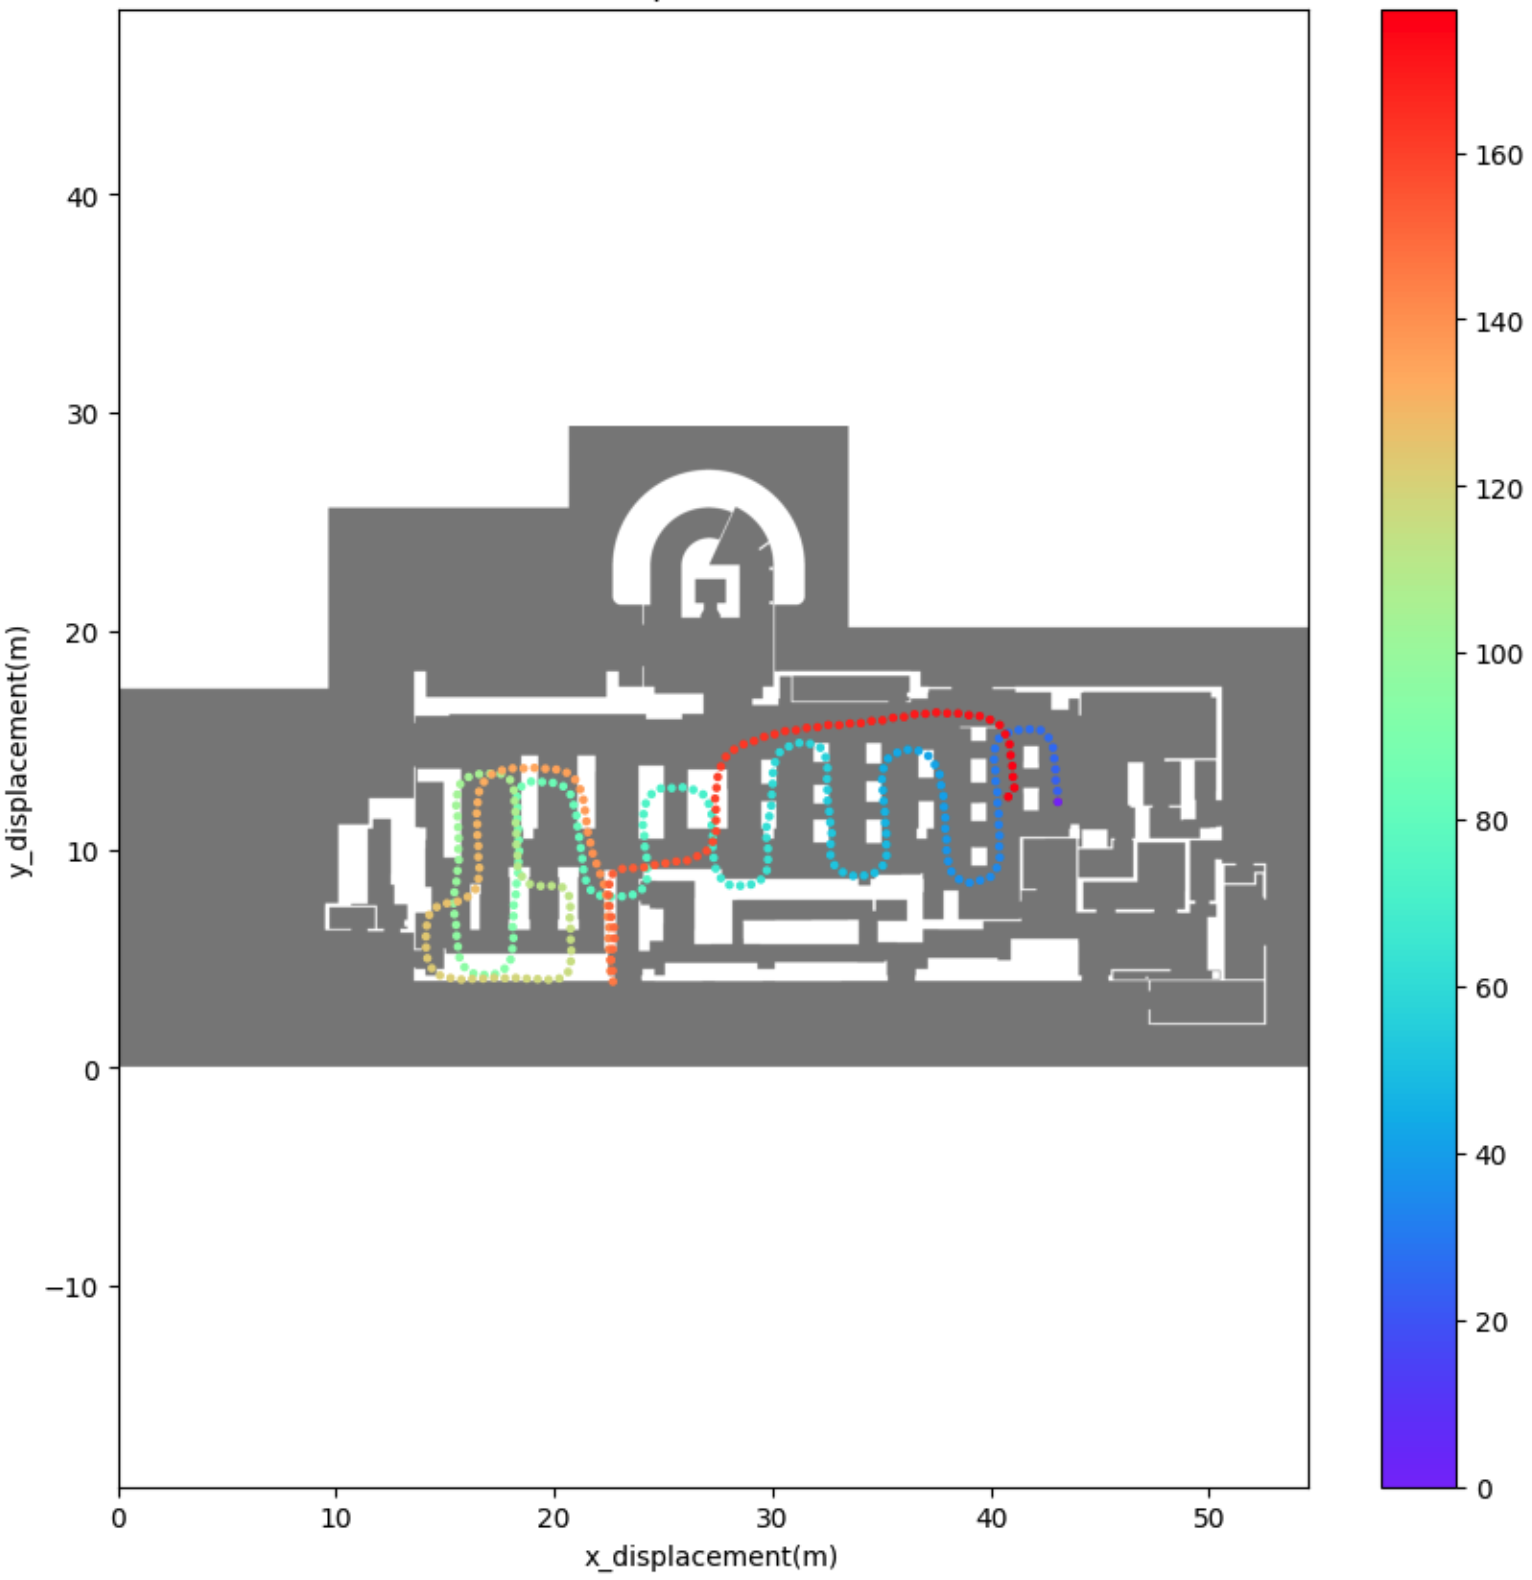
\includegraphics[width=80mm]{image/fingerprint-rotate.jpg}
	\caption{BLEのFPを補正後の軌跡}    \label{fig:fingerprint-rotate}
\end{figure}

\begin{lstlisting}[caption={BLEビーコンのFPを使用した\\初期進行方向補正}, label=lst:rotate-trajectory-using-ble-fingerprint]
def rotate_trajectory_to_optimal
          _alignment_using_ble_fingerprint(
    acc_df: pd.DataFrame,
    angle_df: pd.DataFrame,
    ble_scans_df: pd.DataFrame,
    ble_fingerprint_df: pd.DataFrame,
    floor_name: str,
    *,
    ground_truth_first_point: dict[Axis2D, float] | None = None,
) -> tuple[pd.DataFrame, pd.DataFrame]:                                        
\end{lstlisting}


\ref{fig:pdr-rotate}に示す軌跡の問題点として人間が歩行不可能領域を通過している点がある.
現実の人間がこのような場所を通過しないため,このような軌跡は不適切である.
そのため軌跡が歩行不可領域に存在する場合は,歩行可能な領域に移動させる処理が必要である.
この問題を解決する処理としてListing\ref{lst:map-matching}に示すマップマッチング補正関数を提供する.
マップマッチング補正関数は加速度DF,角度DF,フロアマップ情報DICT,フロア名,及びマップの1pxあたりの距離を受け取る必要がある.
戻り値は時間経過に伴う2次元座標のDFのみを返す.内部の処理の関係上補正後の角度DFは返すのが難しいためである.
関数内部ではまず加速度と角度のデータを基にして軌跡を推定する.
この軌跡に対して,各地点での座標が与えられたフロアマップ上の歩行可能な領域に存在するかどうかを検証する.
検証の結果,各地点での座標が歩行不可能な領域に存在する場合,当該座標から最も近い歩行可能な座標を幅優先探索アルゴリズムを
用いて探す.
該当する座標が見つかった場合,該当座標と該当座標以降の軌跡の座標を歩行可能な座標に平行移動して補正を行う.
当該座標の補正が終了後,次の座標に対して同様の処理を行う処理を繰り返す.
これによって軌跡の各地点が歩行可能な領域に存在するようになり,軌跡全体が最適化される.
図\ref{fig:map-matching}に示すように,マップマッチング補正後の軌跡では
歩行不可能な領域に存在していた地点が歩行可能な地点に移動されている.

\begin{lstlisting}[caption={マップマッチング補正}, label=lst:map-matching]
def move_unwalkable_points_to_walkable(
    acc_df: pd.DataFrame,
    angle_df: pd.DataFrame,
    map_dict: dict[str, np.ndarray],
    floor_name: str,
    dx: float,
    dy: float,
    *,
    ground_truth_first_point: dict[Axis2D, float] | None = None,
) -> pd.DataFrame:

\end{lstlisting}

\begin{figure}[h]
	\centering
	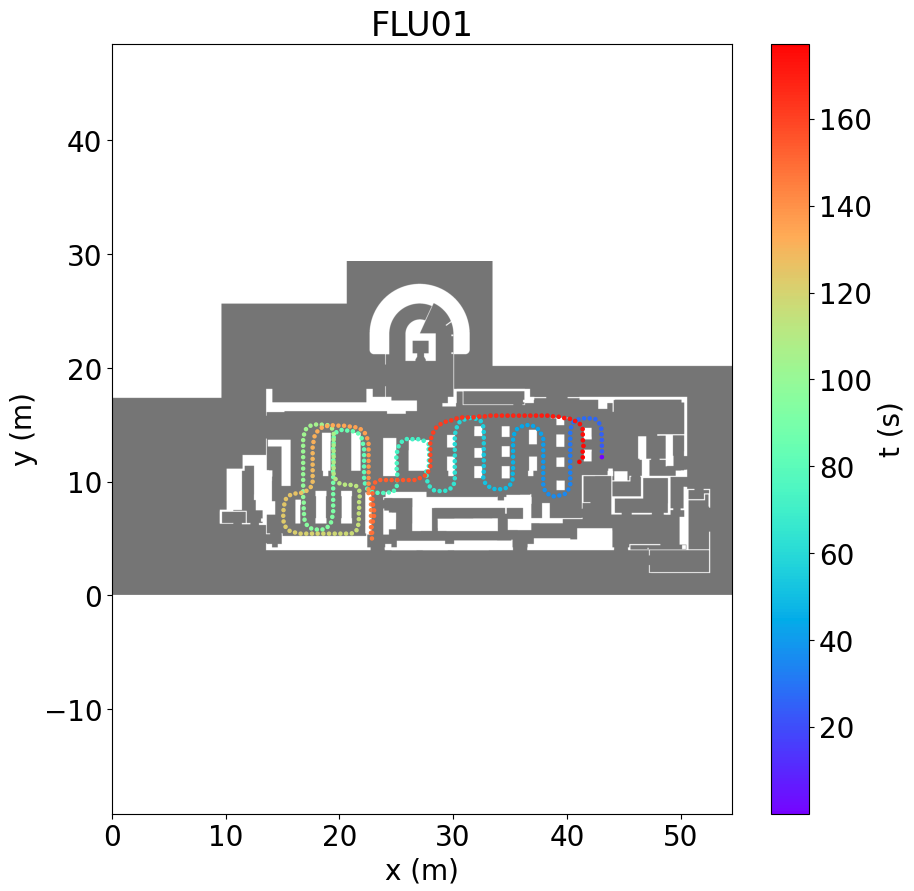
\includegraphics[width=80mm]{image/map-matching.png}
	\caption{マップマッチング補正後の軌跡}    \label{fig:map-matching}
\end{figure}



